\documentclass[11pt]{scrartcl}

\usepackage[T1]{fontenc}
\usepackage[utf8]{inputenc}
\usepackage{lmodern}
\usepackage[english]{babel}
\usepackage{xcolor}
\usepackage{amsmath}
\usepackage{amssymb}
\usepackage{amsfonts}
\usepackage{amsthm}
\usepackage[centerdot]{mathtools}
\usepackage{hyperref}
\usepackage{tikz}
\usepackage[ruled]{algorithm2e}
\SetKw{Continue}{continue}
\SetKw{Null}{null}
\SetKw{Break}{break}
\usepackage[textsize=tiny]{todonotes}
\usepackage[normalem]{ulem}
\usepackage{float}
\usepackage{subfig}

\usepackage{subfig}

\newcommand{\daniel}[1]{\todo[linecolor=blue,backgroundcolor=blue!25]{#1}}
\newcommand{\david}[1]{\todo[linecolor=orange,backgroundcolor=orange!25]{#1}}
\newcommand{\laura}[1]{\todo[linecolor=green,backgroundcolor=green!25]{#1}}
\newcommand{\moritz}[1]{\todo[linecolor=red,backgroundcolor=red!25]{#1}}
\newcommand{\changedByLP}[1]{\textcolor{green!50!black}{#1}}
\newcommand{\changedByDP}[1]{\textcolor{blue!50!black}{#1}}
\newcommand{\changedByDK}[1]{\textcolor{orange!50!black}{#1}}
\newcommand{\changedByMW}[1]{\textcolor{red!50!black}{#1}}

\DeclareMathOperator{\cost}{cost}

%\numberwithin{equation}{section}
\newtheorem{theorem}{Theorem}[section]
\newtheorem{lemma}[theorem]{Lemma}
\newtheorem{definition}[theorem]{Definition}
\newtheorem{property}[theorem]{Property}

\title{Pool Trading for Hybrid Wind-Solar Power Producers}
%alternative: The all optimal integer flow problem and its applications.
\author{David K\"onen, Daniel Piersig, Laura Poreschak, Moritz Wegener  }  % in alphabetical order
%\keywords{All integer optimal flow problem; networkflow; minimum cost flow problem}


\begin{document}

\maketitle

\begin{abstract}
  Blalba    \changedByDK{ mit changedby werden Änderungen in eurer Farbe angezeigt. } 
\end{abstract}

 %Section1
 \section{Introduction}

Renewable energies are currently advancing and gaining an increasing share of the energy production. On the one hand, this is induced by the desire to decrease the carbon footprint and on the other hand, the population is facing a decreasing availability of fossil fuels like natural gas, coal and oil. The advantage of renewable energies is that apart from not requiring fuel, which induces zero fuel costs, it is emission-free and therefore supported by the government. However, these energy sources are also non-dispatchable and have the major disadvantage of uncertainty. Conejo et al. \cite{Conejo10} considered the case of a wind power producer. Due to the uncertainty, the wind power producer must rely on the energy traded on the balancing market. Therefore, he solved an optimisation problem to maximise the expected profits from trading on the day-ahead market and the adjustment market while also minimising the costs incurred in the balancing market caused by energy deviations. 

In addition to the uncertainty, the wind power producer also faces a substantial fluctuation in production throughout the year, caused by the strong dependence on wind availability over different months in a year. Considering a wind power producer in Europe, wind availability is much higher in the winter than summer months, see, e.g. \cite{W11}. 

For this case study, we consider the case of an energy producer producing both wind power as well as solar energy. Several studies have been carried out to see how both resources' production variability  can be decreased by exploiting the anti-correlation of wind speed and solar irradiance. Coker et al. \cite{Coker2013} considered a region in south-west Britain to assess the variability of wind, solar and tidal current energy resources. Santos-Alamillos et al. \cite{Santos-Alamillos} aimed at finding the optimal spatial distribution of wind and solar farms across the Southern Iberian Peninsula to minimise the resulting net variability. Bett et al. \cite{BETT16} analysed daily data for Great Britain and found  evidence for an overall anticorrelation between wind speed and solar irradiance. As a side product, they also discovered that solar variability is significantly higher than wind variability and that both variabilities are higher in winter than in summer. Inspired by these results, we wish to set up a pool trading model for an energy producer offering energy produced from both solar and wind power plants.  
This setting of a hybrid wind-solar power producer
	overcomes the strong fluctuation in production throughout the year due to the strong over year anti-correlation of wind speed and solar irradiance, see figure \ref{fig:overyear}. In addition to
	the anti-correlation between wind speed and solar irradiance over the whole year, there is also an anti-correlation between both over the day, even if it is much smaller. We will exploit this anti-correlation over the day and include it into the forecast
	for wind and solar power production. Therefore, we will apply the forecast for wind power production for a time $t$ in dependence on the previous times' wind speeds and previous times' solar irradiance to improve the forecast precision possibly.

	
\begin{figure}[h!]
	\centering
	
	\begin{minipage}{0.8\textwidth}
		\subfloat{
			\centering
			\scalebox{0.4}{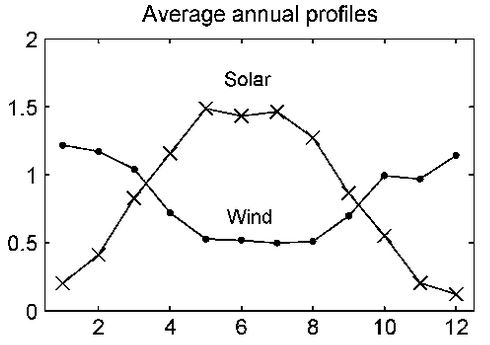
\includegraphics{Figures/year.jpg}}
		}
		\hfill
		\subfloat{
			\centering
			\scalebox{0.4}{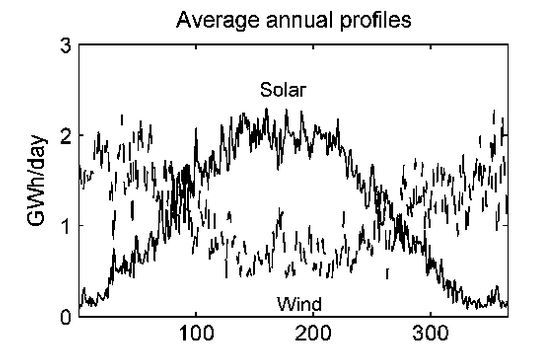
\includegraphics{Figures/year2.png}}
		}
		
		\caption{The average annual profiles of solar irradiance and wind speed \cite{W11}}\label{fig:overyear}
	\end{minipage}	
\end{figure}
To solve the  decision problem, the hybrid energy producer has to face, we will solve a scenario-based multi-stage optimization problem. For generating wind and solar power scenarios, we will use a time-series-based approach on a historical data set. With the generated data, we consider two cases. First, we look at a situation where we do not have an adjustment market. Second, we add an adjustment market to our situation. We compare the revenue of a hybrid producer with the sum of the revenues of a solar and a wind power producer. Our results show that the more risk averse a producer is, the more profitable it is to produce in a hybrid scheme. This effect can be observed in both market situations. We conclude that this profitability stems from the anit-correlation of the two weather conditions as a decrease in availability of solar irradiance is most likely to be compensated by an increase of wind speed and vice versa. This gives more planning security and therefore a higher expected profit. Moreover, the decrease in planning insecurity also explains why more risk averse producers profit more from a hybrid production scheme.  

 
 
 %Section 2 Preliminaries
 \section{Decision framework}
In the introduction we mentioned the three major trading places for energy, namely the day-ahead, the adjustment and the balancing market. All three of these are cleared in a single auction process, however at different times of the day. 

\begin{list}{$\cdot$}{}
	\item The day-ahead market is cleared at a given time period $t^D$ of day $d-1$.
	\item The adjustment market is cleared at time period $t^{A}$ of day $d-1$. Please note that time period $t^{A}$ takes place \textit{after} time period $t^{D}$.
	\item The balancing market ensures the real-time balancing between the generation of and demand for energy by balancing out differences between the real-time operation and the last energy program settled on in the previous markets. Therefore, it is cleared just before each time period of day $d$. 
\end{list}
There are three major decision the hybrid energy producer has to face. First, he has to submit an offering curve to the day-ahead market for each time period of day $d$. Then, he has to modify the submitted energy offers in the adjustment market depending on how the wind and solar power forecast updates change. Finally, he balances out his energy deviations by trading in the balancing market for each time period of day $d$. From now on, we assume hourly periods. This means that the balancing market for the time period 6.00-7.00 am of day $d$ closes at 5.50 am of day $d$. 
\\
\\ The producer faces several factors that influence his short-term decision making process. It is inevitable to account for the imbalance costs, i.e. the costs entailed bx deviations in the energy production. Apart from that, he is influenced by all sorts of mechanisms through which energy deviations are priced in the balancing market and the beneficial impact of an adjustment market clearing after the clearance of the day-ahead market. Energy deviations are not unusual for producers of non-dispatchable energy sources as windspeed and solar irradiance exert a high variability. As soon as a producer deviates from his agreed-upon amount of energy he had traded on the market before, he has to sell its surplus or buy his generation deficit at an \textit{imbalance price}. We denote the price for positive energy deviations, i.e. higher production than planned, by $\lambda_{t}^{+}$ and the price for negative energy deviations by $\lambda_{t}^{-}$. If the producer faces a negative system imbalance $\delta_{t}$, which means there is a deficit of energy generation, we have
\begin{align*}
	&\lambda_{t}^{+}=\lambda_{t}^{D}
	\\ &\lambda_{t}^{-}=max\left(\lambda_{t}^{D}, \lambda_{t}^{UP}\right),
\end{align*}
where we write $\lambda_{t}^{D}$ for the day-ahead market price and $\lambda_{t}^{UP}$ for the price of the upward energy that needs to be added to the system. In case of a generation excess in the power system, i.e. $\delta_{t}>0$, we have 
\begin{align*}
	&\lambda_{t}^{+}=min\left(\lambda_{t}^{D}, \lambda_{t}^{DOWN}\right)
	\\ &\lambda_{t}^{-}=\lambda_{t}^{D}.
\end{align*} 
Here, $\lambda_{t}^{DOWN}$ is the parameter for the price of the downward energy that has to be removed from the system. 
\\ \\
The producer offers an amount $E_{t}^{D}$ of energy at the day-ahead market, while his plant produces an emount $E_{t}$, which is most probably not equal to the amount offered at the day-ahead market. Hence, he expects a revenue of
\begin{equation*}
	R_{t}=\lambda_{t}^{D}\cdot E_{t}^{D} + I_{t},
\end{equation*}
where we write $I_{t}$ for the imbalance income. Note that this can be either positive or negative depending on the market imbalance and the production imbalance. We denote the total deviation by
\begin{equation*}
	\Delta_{t}=E_{t}-E_{t}^{D}=d_{t}\left(P_{t}-P_{t}^{D}\right)
\end{equation*}
indicating the timespan by $d_{t}$ and the actual resp. offered amount of power by $P_{t}$ resp. $P_{t}^{D}$. Applying this notation, we can write
\begin{align*}
	I_{t}= \begin{cases}
		\lambda_{t}^{+}\Delta_{t} &\mathrm{\; if \;} \Delta_{t} \geq 0,
		\\ \lambda_{t}^{-}\Delta_{t} &\mathrm{\; if \;} \Delta_{t}\leq 0
	\end{cases}
\end{align*}
and define the ratios 
\begin{equation*}
	r_{t}^{+}= \frac{\lambda_{t}^{+}}{\lambda_{t}^{D}} \mathrm{\; and \;} r_{t}^{-}=\frac{\lambda_{t}^{-}}{\lambda_{t}^{D}}.
\end{equation*}
Thus, the revenue can be rewritten as
\begin{align*}
	R_{t}= \begin{cases}
		\lambda_{t}^{+}\left(E_{t}\right)+\lambda_{t}^{D}r_{t}^	{+}\Delta_{t} &\mathrm{\; if \;} \Delta_{t} > 0,-\Delta_{t}
		\\ \lambda_{t}^{+}\left(E_{t}\right)+\lambda_{t}^{D}r_{t}^	{-}\Delta_{t} &\mathrm{\; if \;} \Delta_{t}< 0
	\end{cases}
\end{align*} 
In general, we can also formulate the revenue in terms of the maximum level of revenue, which could be realised in a situation free of wind and irradiance uncertainty, and the imbalance cost, which we define as $C_{t}$
\begin{equation*}
	C_{t}=\begin{cases}
		\lambda_{t}\left(1-r_{t}^{+}\right)\Delta_{t} &\mathrm{\; if \;} \Delta_{t}>0
		\\ -\lambda_{t}^{D}\left(r_{t}^{--1}\right)\Delta_{t} &\mathrm{\; if \;} \Delta_{t}<0.
	\end{cases}
\end{equation*}
This characterisation renders it possible to give a more concise formulation of the revenue 
\begin{equation*}
	R_{t}=\lambda_{t}^{D}E_{t}-C_{t},
\end{equation*}
which makes it easy to deduce that maximising the revenue is equivalent to minimising the imbalance costs. 
\\ \\
We face four major sources of uncertainty. The most essential source of uncertainty is the weather, which influences both the wind and solar power generation. Apart from that, we have uncertainty concerning the market characteristics like day-ahead market price, adjustment market price and the prices for imbalance.
For our purpose, we consider $N_{T}$ periods of the market horizon, $N_{D}$ scenarios for day-ahead prices and $N_{A}$ scenarios for the adjustment market prices. Thus, we have several realisations of day-ahead and adjustment market prices, which we summarise in
\begin{align*}
	\lambda^{D}=\left\{\lambda_{t}^{D} \quad \lvert \quad t \in \left\{1, .., N_{T}\right\}\right\}
	\\ \lambda^{A}=\left\{\lambda_{t}^{A}\quad \lvert \quad t \in \left\{1, .., N_{A}\right\}\right\}.
\end{align*}
The hybrid power producer has to adhere the following sequence of decisions. First, the designs an offer strategy for the day-ahead market and submits his selling offers for each period of the market horizon. Second, once the day-ahead market is known for each time period, he has to decide on the amount of energy that he wishes to sell or buy from the adjustment market. As soon as the adjustment market prices are known as well as the imbalance prices and the generated wind and solar power, the producer knows his level of imbalance and can compute the resulting costs for the latter.  


 %Section 3 Theoretical Foundations
 %\input{}

 
 %Section 4 All Optimum Flow Algorithm 
 %\input{} 
 

 %Section 5 
 %\input{} 
 
 

 %Section 6
 %\input{}
 

 %\section{Applications}

 %kann man auch in den Motivation-Abschnitt reinwurschteln

 %\section{Computational Results}

 %Aus der MA kopieren

 %\section{Conclusion}

 %blablablablabla

 \bibliographystyle{plain}
 \bibliography{libary}


\end{document}
